\documentclass[
	aspectratio=169, 
	10pt 
]{beamer}
\usepackage[utf8]{inputenc} 
\usepackage[ngerman]{babel}

\usepackage{fancybeamer} 
\usepackage{../vendor/fancyqr/fancyqr}
\usepackage{../vendor/tikzpingus/tex/tikzpingus}

\usepackage{listings}
\usepackage{graphicx}
\usepackage{tikz}
\usetikzlibrary{decorations.pathreplacing} 
\usetikzlibrary{arrows,decorations.markings}
\usetikzlibrary{shapes.geometric}
\usetikzlibrary{backgrounds,arrows.meta}
\usepackage{fontawesome}

%%%%%%%%%%%%%%%%%%%%%%%%%%%%%%%%%%%%%%%%%%%%%%%%%%%%%%%%%%%%%%%%%%%%%%
%\annotatedFigureBoxCustom{bottom-left}{top-right}{label}{label-position}{box-color}{label-color}{border-color}{text-color}
\newcommand*\annotatedFigureBoxCustom[8]{\draw[#5,thick,rounded corners] (#1) rectangle (#2);\node at (#4) [fill=#6,thick,shape=circle,draw=#7,inner sep=2pt,font=\sffamily,text=#8] {\textbf{#3}};}
%\annotatedFigureBox{bottom-left}{top-right}{label}{label-position}
\newcommand*\annotatedFigureBox[4]{\annotatedFigureBoxCustom{#1}{#2}{#3}{#4}{black}{white}{black}{black}}
\newcommand*\annotatedFigureText[4]{\node[draw=none, anchor=south west, text=#2, inner sep=0, text width=#3\linewidth,font=\sffamily] at (#1){#4};}
\newenvironment {annotatedFigure}[1]{\centering\begin{tikzpicture}
    \node[anchor=south west,inner sep=0] (image) at (0,0) { #1};\begin{scope}[x={(image.south east)},y={(image.north west)}]}{\end{scope}\end{tikzpicture}}
%%%%%%%%%%%%%%%%%%%%%%%%%%%%%%%%%%%%%%%%%%%%%%%%%%%%%%%%%%%%%%%%%%%%%%

\pgfdeclarelayer{background}\pgfdeclarelayer{foreground}\pgfdeclarelayer{middle}
\pgfdeclarelayer{very-background}
\pgfsetlayers{very-background,background,main,middle,foreground}

\title{How-To-Studium} % short title is used for the slide footer but optional
\author{Lars Pfrenger} % short author title is used for the slide footer but optional
\date{07. Oktober 2024} 

\begin{document}

\maketitle[assets/uni.png][50] % title slide with optional title picture and parameter to move it upwards

\begin{frame}{Willkommen}
    \centering
    \begin{tikzpicture}
        \pingu[graduate,eyes wink, wings wave,graduate tassel]
     \end{tikzpicture}%

\end{frame}

\begin{frame}{Links}
    \begin{fancycolumns}[widths={40,40}]
        \fancyqr[image = \huge\faGithub, height=\linewidth]{https://github.com/FIN-Uni-Ulm/how-to-studium}
        \nextcolumn
        \fancyqr[height=\linewidth]{https://www.uni-ulm.de/in/fakultaet/studium/fachbereich-informatik/fuer-studierende}
    \end{fancycolumns}
    
    \begin{fancycolumns}[widths={40,40}]
        \begin{center}
            Source \& PDF Download
        \end{center}
        \nextcolumn
        \begin{center}
            Übersichtsseite der Uni
        \end{center}

    \end{fancycolumns}
\end{frame}



\section{Übersicht}

\subsection{Was ist ein Modul}
\begin{frame}{\insertsubsection}
    \begin{fancycolumns}[columns=2]
        \begin{definition}{Vorlesung}
            Dozent/-in steht im Hörsaal und lehrt über ein Themengebiet
        \end{definition}
        
        \begin{definition}{Übung}
            \begin{itemize}
                \item Übungsblätter
                \item Notenbonus oder Vorleistung für Prüfung
                \item Prüfungsrelevant
                \item Abgabe erfolgt über Moodle
            \end{itemize}
        \end{definition}
        
        \nextcolumn
        \begin{definition}{Tutorien}
            \begin{itemize}
                \item Von anderen Studierenden gehalten
                \item Besprechung der Übungsblätter 
                \item Tipps, weitere Übungsaufgaben
                \item Anmeldung über Moodle
            \end{itemize}
        \end{definition}

        \begin{definition}{Prüfung}
            \begin{itemize}
                \item Meist schriftliche Klausur
                \item Aber auch mündliche Prüfungen, etc
            \end{itemize}
        \end{definition}

    \end{fancycolumns}
\end{frame}

\subsection{Studienplan}
\begin{frame}{\insertsubsection}
    \begin{fancycolumns}[widths={48}]
        \fancyqr[height=0.8\linewidth]{https://www.uni-ulm.de/in/fakultaet/studium/plaene-ordnungen/pruefungsordnungen/}
        \nextcolumn
        \includegraphics[height=0.7\pdfpageheight, trim={1cm 11cm 1cm 2.2cm}, clip]{assets/SP-BA-Inf-FSPO2022.pdf}
    \end{fancycolumns}
\end{frame}

\begin{frame}{\insertsubsection}
    \includegraphics[width=\linewidth, trim={1cm 20.1cm 1cm 2.2cm}, clip]{assets/SP-BA-Inf-FSPO2022.pdf}
\end{frame}

\begin{frame}{\insertsubsection\space(Kategorien)}
    \begin{itemize}
        \item Praktische, Theoretische, Technische Informatik + Mathematik
        \item \textbf{Seminar}, \textbf{ASQ}: Lernen von wissenschaftlicher Arbeitsweise. Seminararbeit + 2 Pflicht ASQ
        \item \textbf{Vertiefungsbereich}: Freie Modulwahl aus dem Vertiefungsbereich 
        \item \textbf{Ergänzungsbereich}: Wahl aus jedem Modul der Uni (so lange nicht eigenes Studienfach, oft aus dem ASQ Bereich)
    \end{itemize}
\end{frame}

\subsection{LP und SWS}
\begin{frame}{\insertsubsection}
    \begin{fancycolumns}[T]

        \begin{definition}{Leistungspunkte (LP / ECTS)\footnotemark[1]}
            \begin{itemize}
                \item Vergabe bei erfolgreichem Abschluss eines Moduls (Prüfung bestanden)
                \item Insgesamt $180$ LP für den Bachelor
                \item $\approx 30$ pro Semester
                \item $1 \text{ LP } \hat{=} \text{ } 30$ Stunden pro Semester
            \end{itemize}
        \end{definition}

        \nextcolumn
        
        \begin{definition}{Semesterwochenstunden (SWS)\footnotemark[2]}
            \begin{itemize}
                \item Anzahl der Stunden, welche ein Modul pro Woche einnimmt
                \item 1 SWS $\hat{=}$ $45$ min
                \item Unterteilt in Vorlesung, Übung und Projekt
            \end{itemize}
        \end{definition}
    \end{fancycolumns}

    \footnotetext[1]{\url{https://www.student.uni-stuttgart.de/uni-a-bis-z/ECTS-Credits-Leistungspunkte/}}
    \footnotetext[2]{\url{https://www.student.uni-stuttgart.de/uni-a-bis-z/SWS--Semesterwochenstunde/}}
\end{frame}


\subsection{Regelstudienzeit}
\begin{frame}{\insertsubsection}
    \begin{itemize}
        \item Plan ist eine Empfehlung. Man kann Module vorziehen oder nach hinten schieben.
        \item Max. 10 Semester
        \item \large\textbf{Aber}: Orientierungsprüfungen beachten! 
    \end{itemize}
\end{frame}
    
\subsection{Orientierungsprüfungen}
\begin{frame}{Orientierungsprüfungen}
    \begin{definition}{Orientierungsprüfungen}
        \begin{itemize}
            \item Prüfungen, welche bis zum Ende des Prüfungszeitraums des 4. Semester bestanden werden müssen. 
            \item Ohne diese darf man nicht weiter studieren.
            \item Wenn die Orientierungsprüfungen bestanden sind, hat man insgesamt \underline{max. 10 Semester} für den Bachelor 
        \end{itemize}
    \end{definition}
\end{frame}


\def\historybox#1#2#3#4{node[history@box,below #1] (@) {\textbf{#2}: #3\ifx!#4!\else\\\footnotesize\itshape#4\par\fi}}
\begin{frame}[c,plain]{\insertsubsection}
  \tikzset{history-line/.style={line width=1.85mm,gray!30!white,line cap=round,rounded corners=2pt},history-event dead/.style={history-event, red}, history-line done/.style={history-line, green}, history-line extra/.style={history-line, blue}, history-line skip/.style={history-line, line width=.75mm,loosely dotted},history-event/.style={history-line,gray,line width=1mm,{Circle[length=1.85mm]}-,shorten <= -1.85mm/2},history@box/.style={yshift=.675\baselineskip,black,text width=5.75cm,font=\small},fakeimg/.style={draw=darkgray,thick,inner sep=0pt}}
  \begin{tikzpicture}
    % \draw[history-line] (0,0)--++(1,0) coordinate (@) ++(1,0) -- ++(1,0) coordinate (@2) ++(1.9,0) -- ++(1,0) coordinate (@3) ++(1,0) -- ++(5,0) coordinate (@4);
    % \pause
    % \draw[history-event] (.25,0) -- ++(.25*.5/1.5,-2.5) -- ++(.25,0) \historybox{right}{March, 17}{The Idea}{asd};
    % \pause
    % \draw[history-event] (.5,0) -- ++(.25*.5/1.5,.75) -- ++(.25,0) \historybox{right}{March, 21 \& 22}{Initial Implementation}{Basic Frontend, Game, Level Format, DSL};
    % \IfFileExists{img/hist-2.png}{%
    %   \node[above right,yshift=1cm,fakeimg] at(.75,0) {\includegraphics[width=4.65cm]{img/hist-2.png}};
    % }{}
    \draw[history-line] (0,0) -- (\linewidth,0);
    \only<2>{\draw[history-line done] (0,0) -- (2.5\linewidth/9,0);}
    \only<3>{\draw[history-line done] (0,0) -- (3.5\linewidth/9,0);}
    \only<4>{
        \draw[history-line done] (0,0) -- (6\linewidth/9,0);
        \draw[history-line extra] (6\linewidth/9,0) -- (9\linewidth/9,0);
    }


    \foreach \x in {1,...,4}
    {
        \draw[history-event]({(\x-1) * \linewidth / 9},0.0) -- ({(\x-1) * \linewidth / 9},-0.5);
        \node[below] at ({(\x-1) * \linewidth / 9},-0.6) {\x};
    }


    \pause
    \draw[history-event dead] (2.5 * \linewidth / 9, 0.0) -- (2.5 * \linewidth / 9, -1.4)
    node[midway,below,yshift=-20pt] {\color{black}Ende der 2. Prüfungsphase des 3. Semesters}
    node[midway,below,yshift=-30pt] {3/4 Prüfungen};


    \pause
    \draw[history-event dead] (3.5 * \linewidth / 9, 0.0) -- (3.5 * \linewidth / 9, 0.8)
    node[midway,above,yshift=+12pt] {\color{black}Ende der 2. Prüfungsphase des 4. Semesters}
    node[midway,above,yshift=+22pt] {4/4 Prüfungen};

    \pause

    \foreach \x in {5,...,10}
    {
        \draw[history-event]({(\x-1) * \linewidth / 9},0.0) -- ({(\x-1) * \linewidth / 9},-0.5);
        \node[below] at ({(\x-1) * \linewidth / 9},-0.6) {\x};
    }


    \end{tikzpicture}
\end{frame}

\subsection{Orientierungsprüfungen (Informatik / Software Engineering)}
\begin{frame}{\insertsubsection \footnotemark[1]}
    \begin{itemize}
        \item Bis zum Ende des Prüfungszeitraums des 3. Fachsemesters mindestens 3 und bis zum Ende des Prüfungszeitraums des 4. Fachsemesters mindestens 4 Modulprüfungen aus der Menge: \begin{itemize}
        \item Grundlagen der Technischen Informatik
        \item Grundlagen der Praktischen Informatik
        \item Grundlagen der der Theoretischen Informatik
        \item Mathematik für Informatik I
        \item Mathematik für Informatik II \end{itemize}
        \item \textbf{Wichtig}: Die meisten Module werden nur im Winter- bzw Sommersemester angeboten
    \end{itemize}

    \footnotetext[1]{{\href{https://www.uni-ulm.de/fileadmin/website_uni_ulm/zuv/zuv.dezIII.abt2u3/3-2oeffentlich/bekanntmachungen/2022/FSPO_Informatikstudiengaenge.pdf}{§ 14 Abs. 1 FSPO}}}
\end{frame}

\subsection{Orientierungsprüfungen (Medieninformatik)}
\begin{frame}{\insertsubsection \footnotemark[1]}
    \begin{itemize}
        \item Bis zum Ende des Prüfungszeitraums des 3. Fachsemesters mindestens 3 und bis zum Ende des Prüfungszeitraums des 4. Fachsemesters mindestens 4 Modulprüfungen aus der Menge: \begin{itemize}
        \item \underline{Grundlagen der Medieninformatik}
        \item Grundlagen der Praktischen Informatik
        \item Grundlagen der der Theoretischen Informatik
        \item Mathematik für Informatik I
        \item Mathematik für Informatik II \end{itemize}
        \item \textbf{Wichtig}: Die meisten Module werden nur im Winter- bzw Sommersemester angeboten
    \end{itemize}

    \footnotetext[1]{{\href{https://www.uni-ulm.de/fileadmin/website_uni_ulm/zuv/zuv.dezIII.abt2u3/3-2oeffentlich/bekanntmachungen/2022/FSPO_Informatikstudiengaenge.pdf}{§ 14 Abs. 2 FSPO}}}
\end{frame}

\subsection{Welche Module im ersten Semester}
\MakeNewBox{gdti}{yellow}
\MakeNewBox{gdtech}{orange}
\MakeNewBox{mathb}{cyan}
\MakeNewBox{gdpi}{pink}

\begin{frame}{\insertsubsection}
    \begin{fancycolumns}
        \begin{gdpi}{} Grundlagen der Praktischen Informatik\newline\end{gdpi}
        \begin{gdti}{} Grundlagen der Theoretischen Informatik\newline\end{gdti}

        \nextcolumn
        \begin{gdtech}{} Grundlagen der Technischen Informatik / \newline Grundlagen der Medieninformatik\end{gdtech}
        \begin{mathb}{} Mathematik für Informatik I\newline\end{mathb}
    \end{fancycolumns}
\end{frame}

\subsection{Wiederholungsversuche}
\begin{frame}{\insertsubsection \space (Informatik)}
    \begin{itemize}
        \item Insgesamt 4 Versuche \footnotemark[1] \begin{itemize} 
            \item Mathematik für Informatik I
            \item Mathematik für Informatik II
            \item Angewandte Numerik
            \item Angewandte Stochastik
            \item Objektorientierte Programmierung \end{itemize}
        \item \textbf{Sonstige Prüfungen}: Insgesamt 3 Versuche
    \end{itemize}

    \footnotetext[1]{\href{https://www.uni-ulm.de/fileadmin/website_uni_ulm/zuv/zuv.dezIII.abt2u3/3-2oeffentlich/bekanntmachungen/2022/FSPO_Informatikstudiengaenge.pdf}{§ 19 Abs. 1 FSPO}}
\end{frame}

\begin{frame}{\insertsubsection \space (Software Engineering)}
    \begin{itemize}
        \item Insgesamt 4 Versuche \footnotemark[1] \begin{itemize} 
            \item Mathematik für Informatik I
            \item Mathematik für Informatik II
            \item Angewandte Stochastik
            \item \underline{Grundlagen der Technischen Informatik}
            \item Objektorientierte Programmierung \end{itemize}
        \item \textbf{Sonstige Prüfungen}: Insgesamt 3 Versuche
    \end{itemize}

    \footnotetext[1]{\href{https://www.uni-ulm.de/fileadmin/website_uni_ulm/zuv/zuv.dezIII.abt2u3/3-2oeffentlich/bekanntmachungen/2022/FSPO_Informatikstudiengaenge.pdf}{§ 19 Abs. 3 FSPO}}
\end{frame}

\begin{frame}{\insertsubsection \space (Medieninformatik)}
    \begin{itemize}
        \item Insgesamt 4 Versuche \footnotemark[1] \begin{itemize} 
            \item Mathematik für Informatik I
            \item Mathematik für Informatik II
            \item Angewandte Stochastik
            \item \underline{Grundlagen der Medieninformatik}
            \item Objektorientierte Programmierung \end{itemize}
        \item \textbf{Sonstige Prüfungen}: Insgesamt 3 Versuche
    \end{itemize}

    \footnotetext[1]{\href{https://www.uni-ulm.de/fileadmin/website_uni_ulm/zuv/zuv.dezIII.abt2u3/3-2oeffentlich/bekanntmachungen/2022/FSPO_Informatikstudiengaenge.pdf}{§ 19 Abs. 2 FSPO}}
\end{frame}

\subsection{Stundenplan}
\begin{frame}{\insertsubsection}
    \begin{fancycolumns}[widths={30}]
        \fancyqr[height=\linewidth]{https://www.uni-ulm.de/fileadmin/website_uni_ulm/iui2/dokumente/Stundenplaene/Stundenplaene-2024-SoSe/2024-WiSe-Stundenplaene_FSPO2022.pdf}
        \nextcolumn
        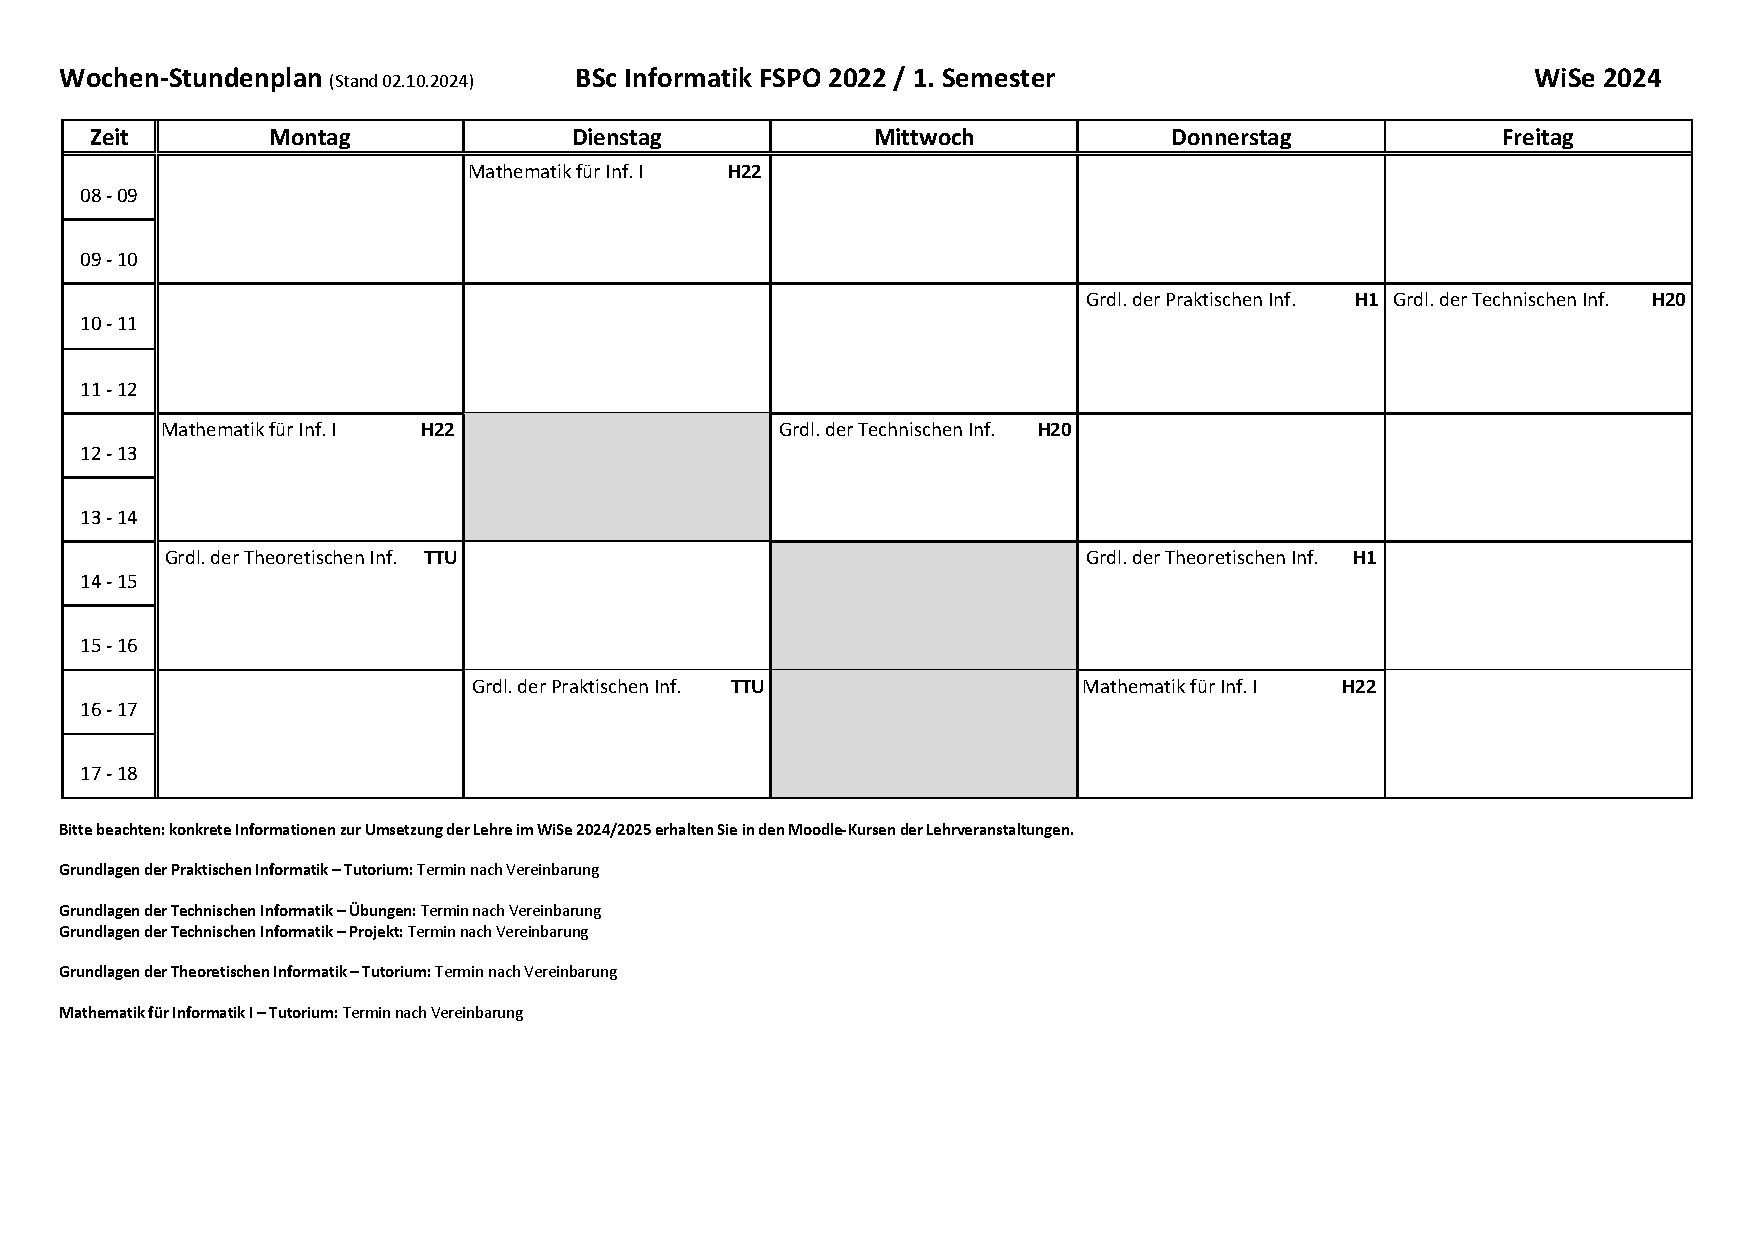
\includegraphics[width=\linewidth, trim={1cm 7.4cm 1cm 2cm}, clip, page=1]{assets/2024-WiSe-Stundenplaene_FSPO2022.pdf}
    \end{fancycolumns} 
\end{frame}


\subsection{Wo bekommt man mehr Infos?}
\begin{frame}{\insertsubsection}
    \begin{itemize}
        \item Campusonline / LSF
        \item CoronaNG
        \item Moodle
        \item E-Mail
        \item Portal / kiz Web-Services
    \end{itemize}
\end{frame}

\subsection{LSF}
\begin{frame}{\insertsubsection \space|\space\underline{\href{https://campusonline.uni-ulm.de}{campusonline.uni-ulm.de}}}
    \begin{itemize}
        \item Prüfungsanmeldung
        \item Transcript of Records
        \item Veranstaltungsverzeichnis
        \item Offizielle Verwaltung!
    \end{itemize}
\end{frame}

\subsection{Wo / Wann finden Module statt?}
\begin{frame}{\insertsubsection \space|\space\underline{\href{https://campusonline.uni-ulm.de}{campusonline.uni-ulm.de}}}
    \begin{annotatedFigure}
        {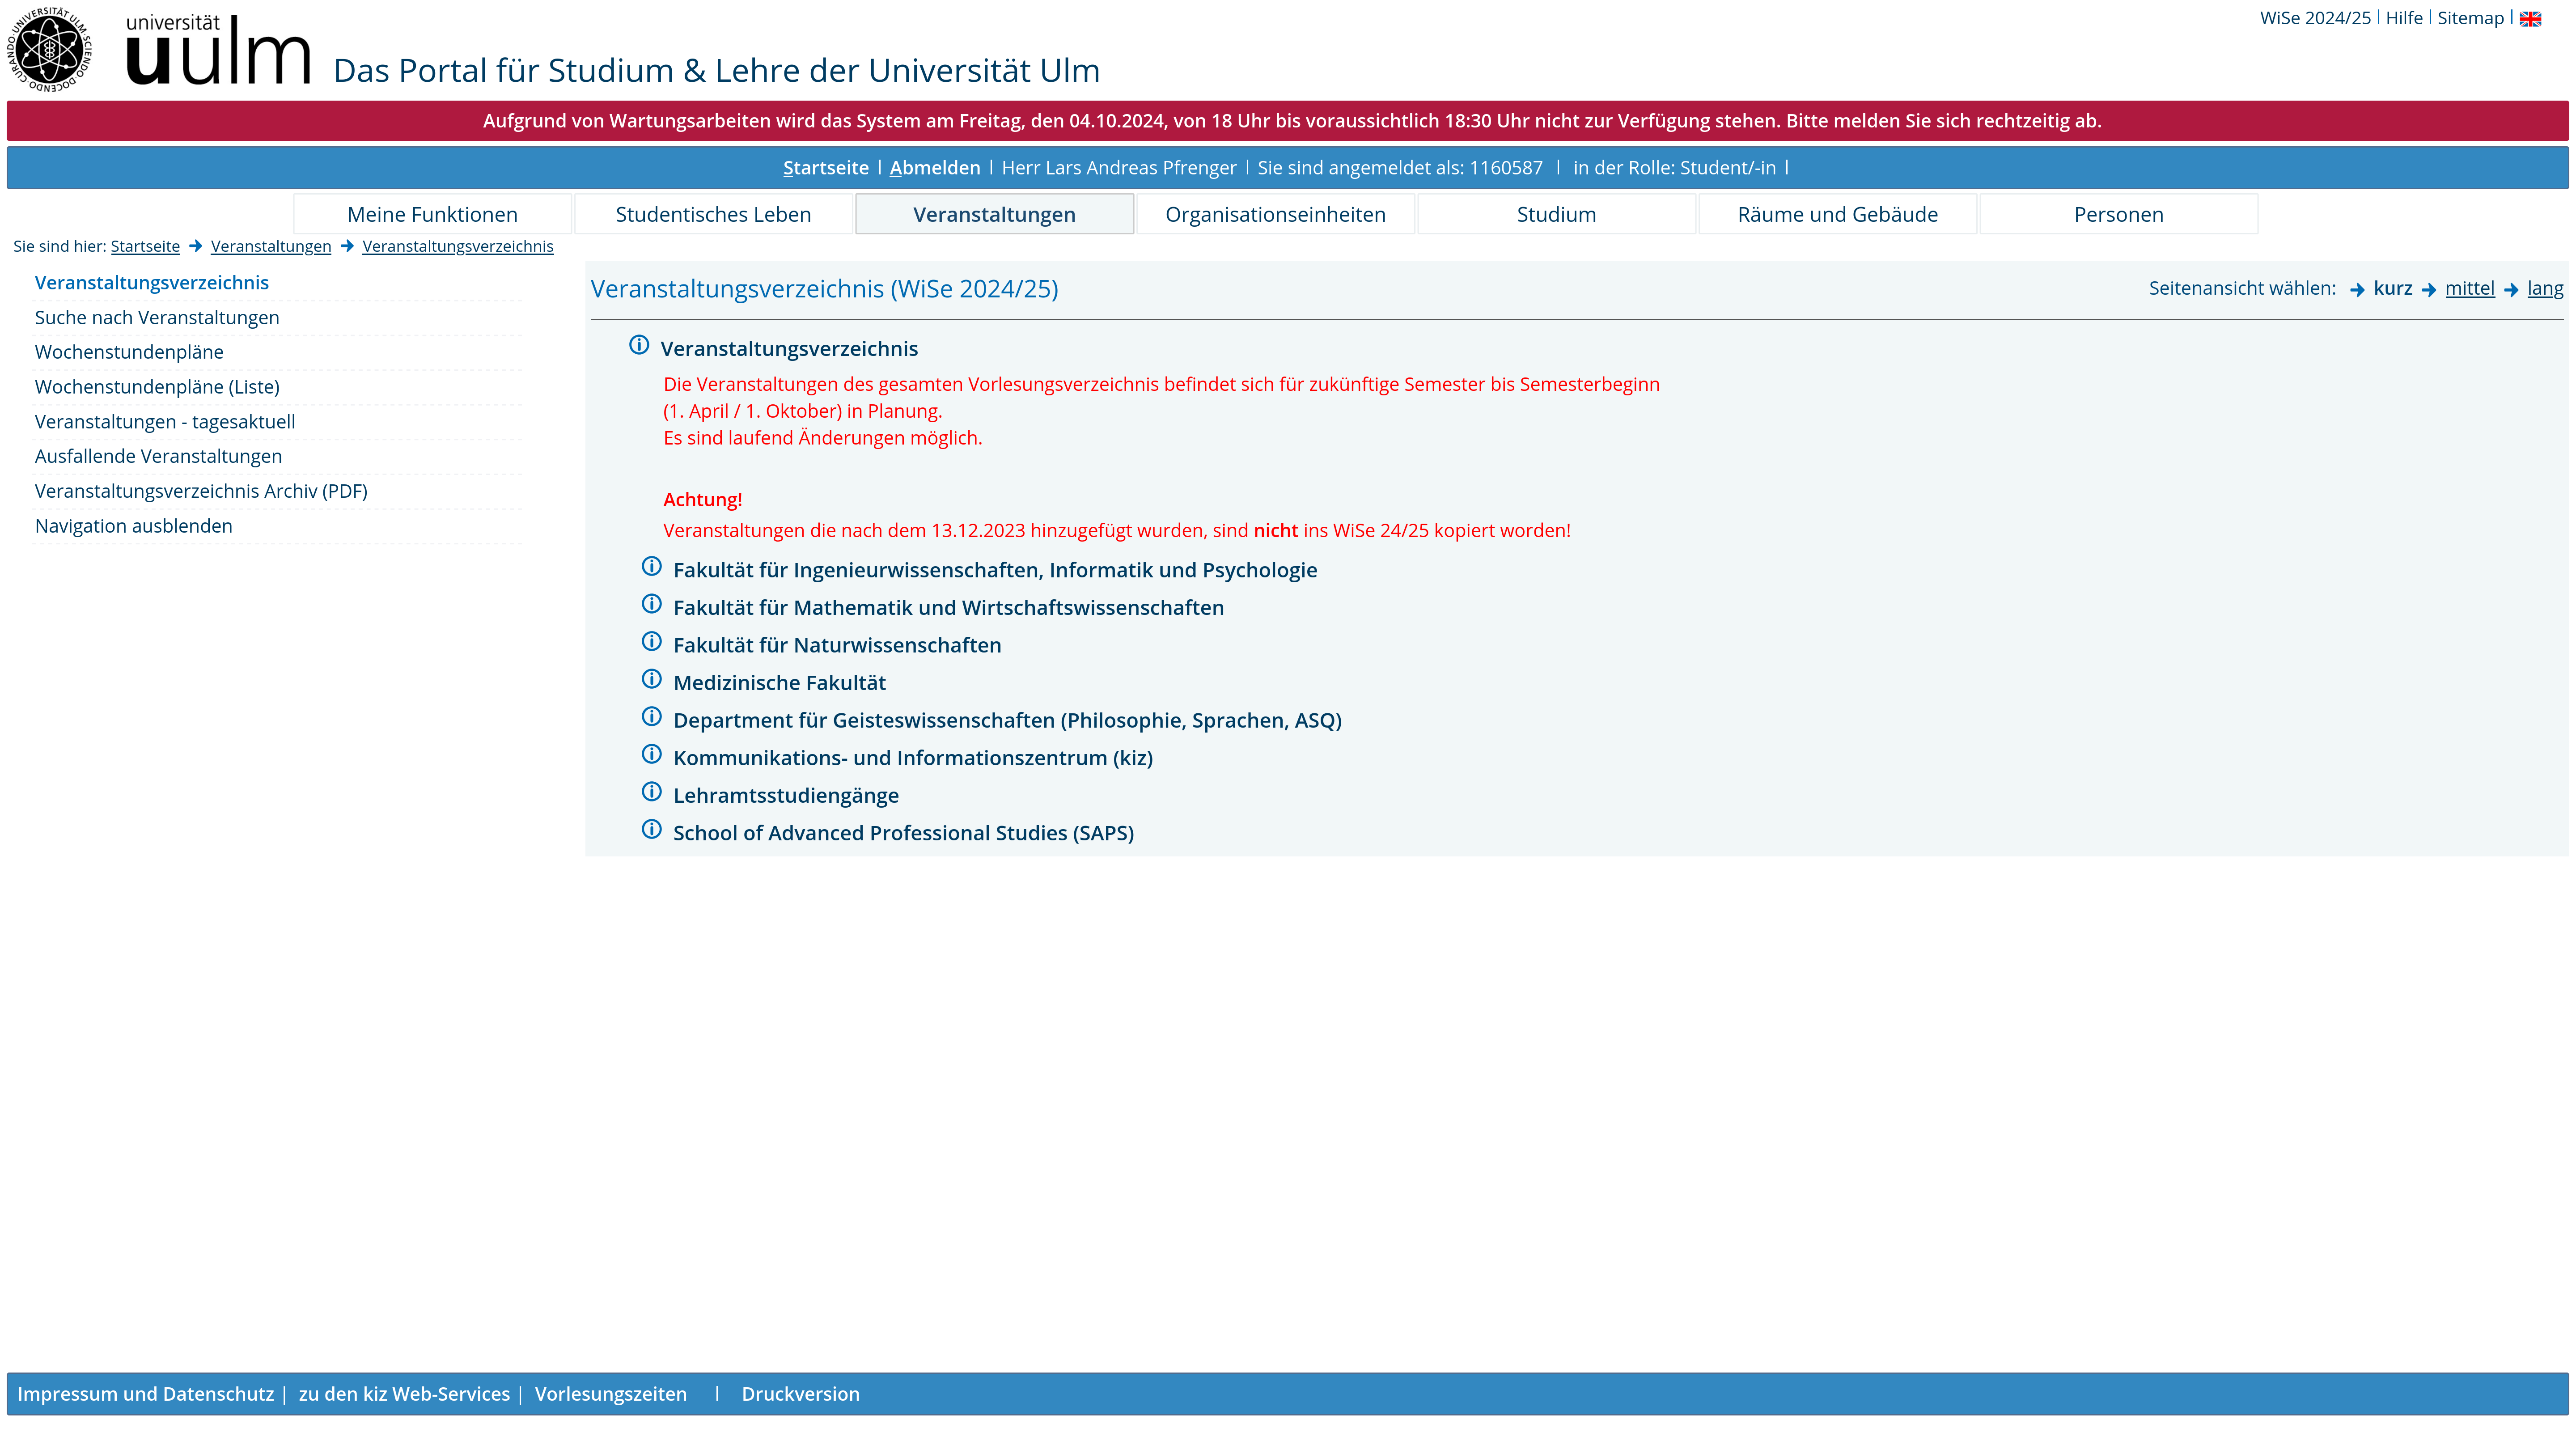
\includegraphics[clip, trim={0 0 0 0}, width=\linewidth]{assets/lsf-1.png}}
        \annotatedFigureBox{0.3328,0.8382}{0.444,0.8654}{A}{0.3328,0.8382}%bl
        \annotatedFigureBox{-0.001,0.7902}{0.111,0.8225}{B}{-0.001,0.7902}%bl
        \annotatedFigureBox{0.231,0.5911}{0.523,0.6268}{C}{0.231,0.5911}%bl
    \end{annotatedFigure}
\end{frame}


\begin{frame}{\insertsubsection \space|\space\underline{\href{https://campusonline.uni-ulm.de}{campusonline.uni-ulm.de}}}
    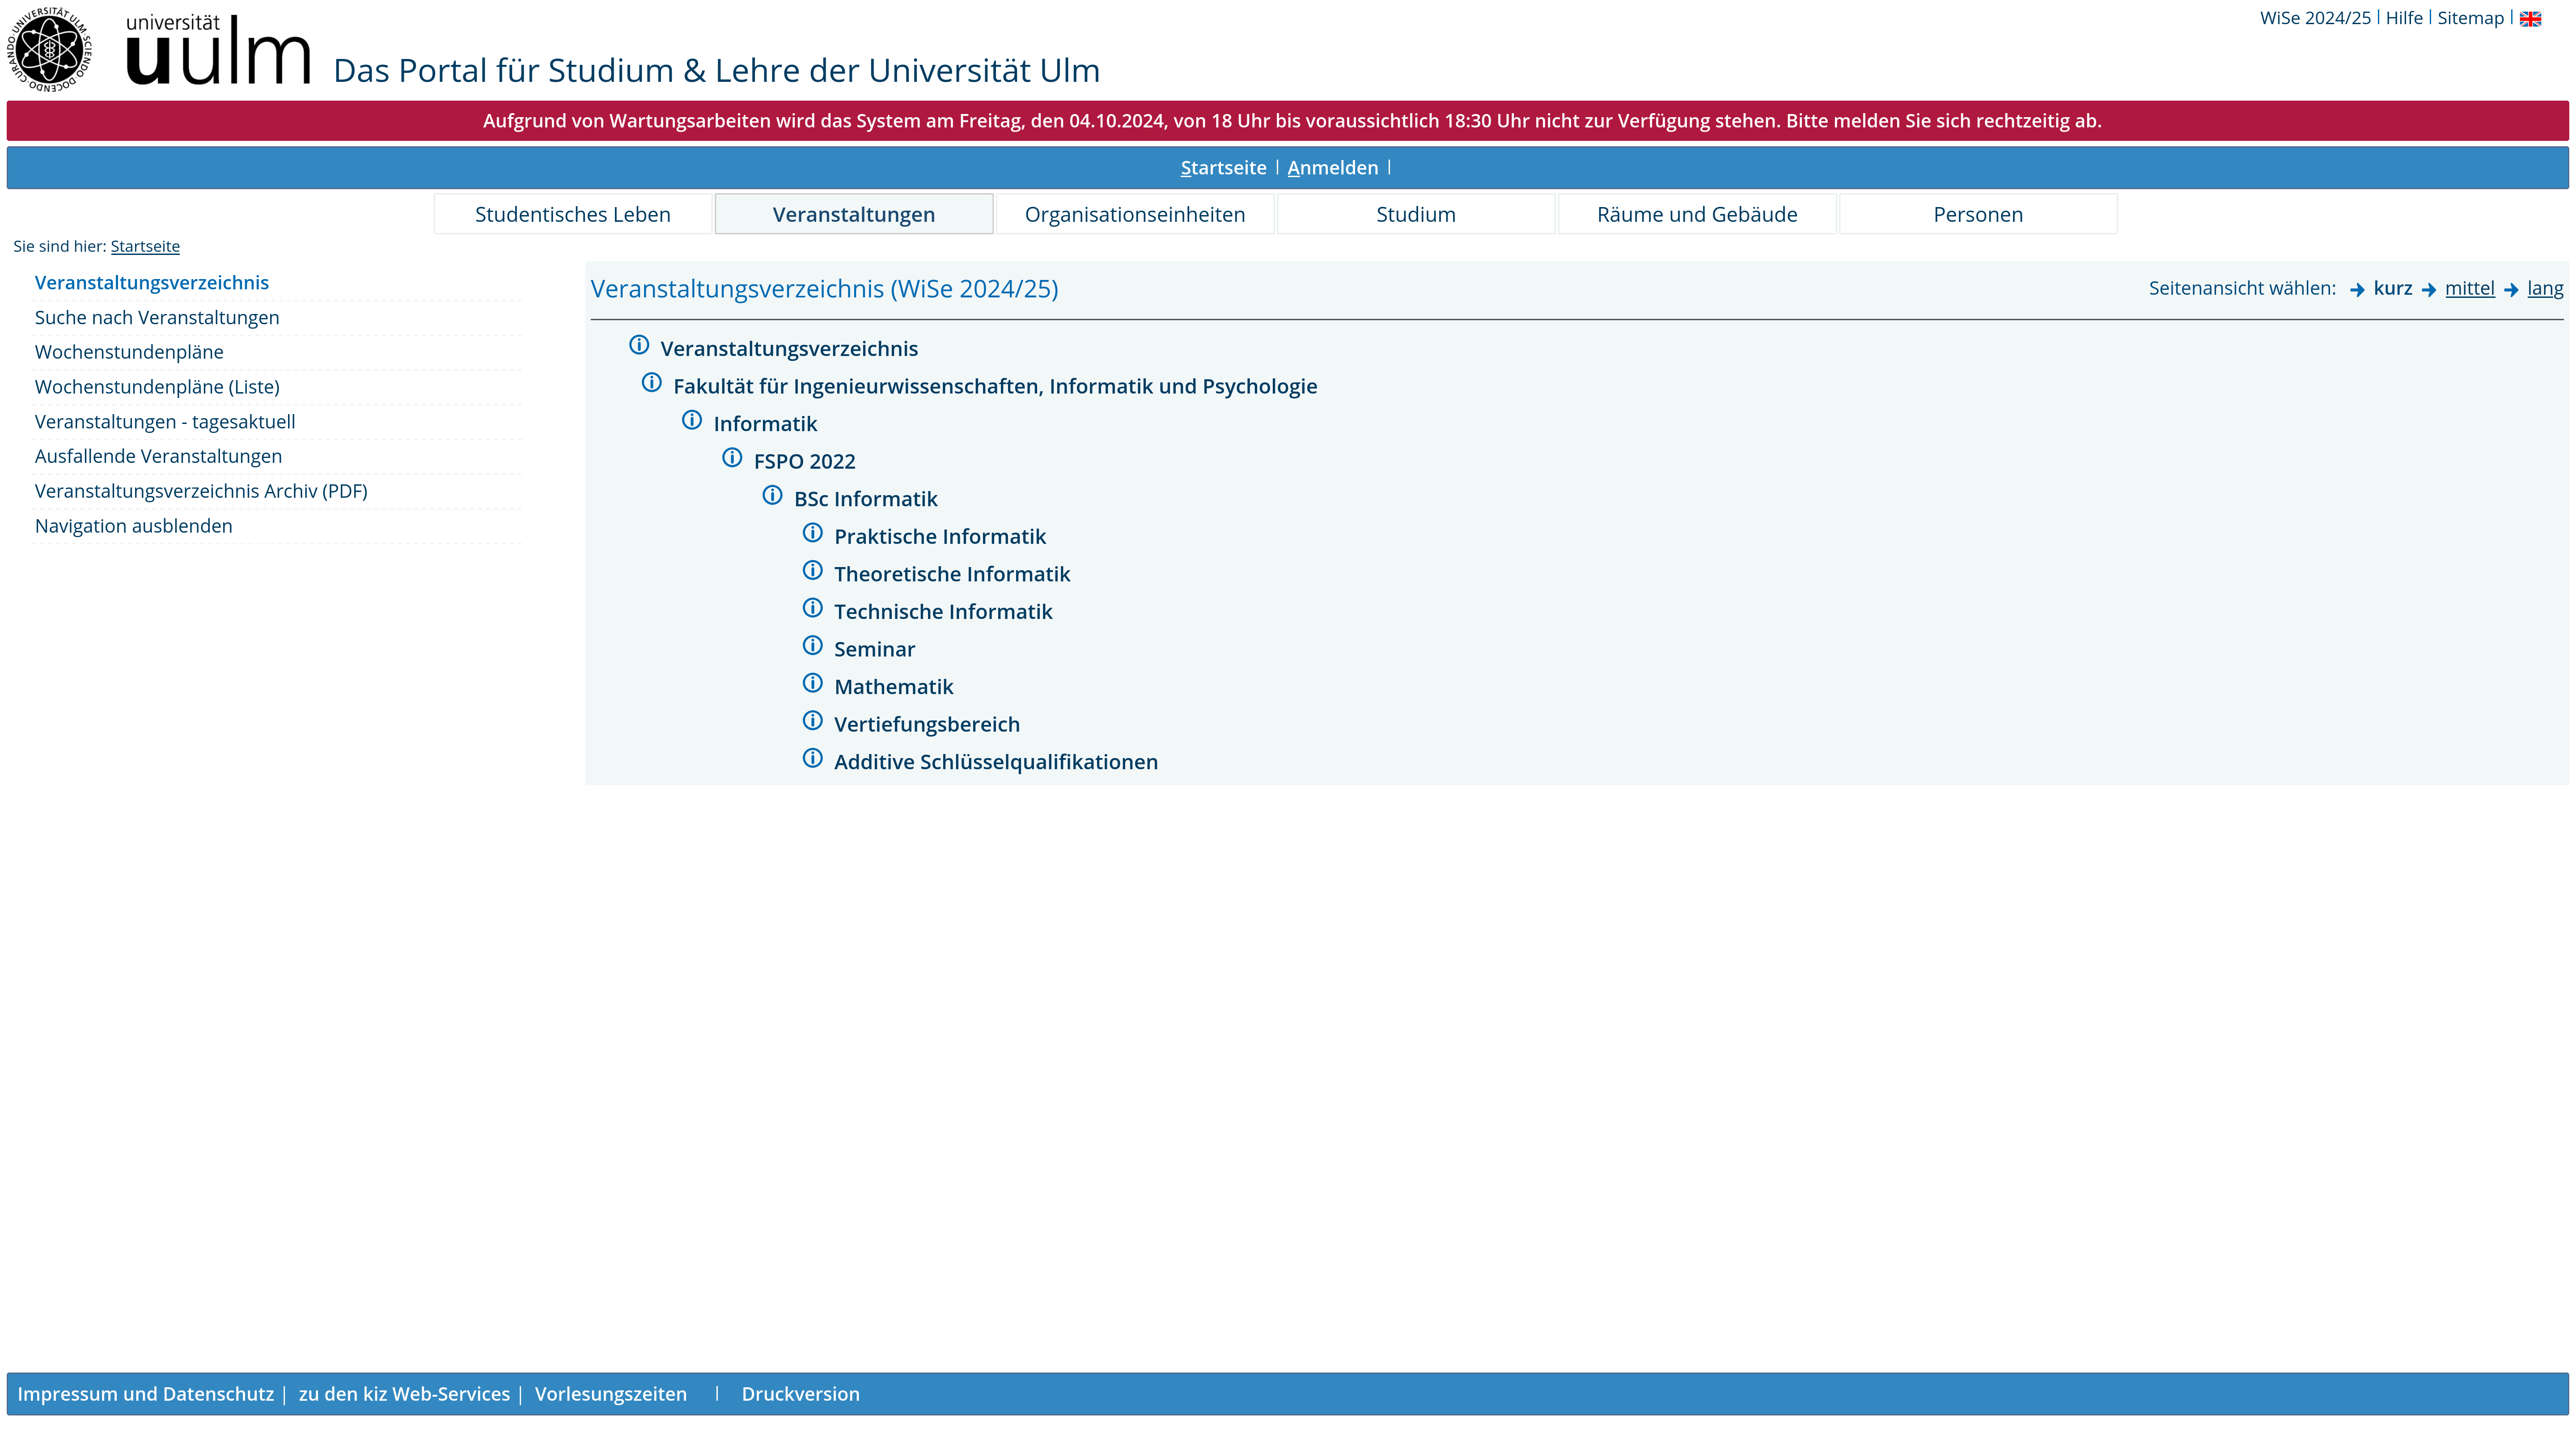
\includegraphics[clip, trim={0 10cm 0 0}, width=\linewidth]{assets/lsf-2.png}
\end{frame}

\begin{frame}{\insertsubsection \space|\space\underline{\href{https://campusonline.uni-ulm.de}{campusonline.uni-ulm.de}}}
    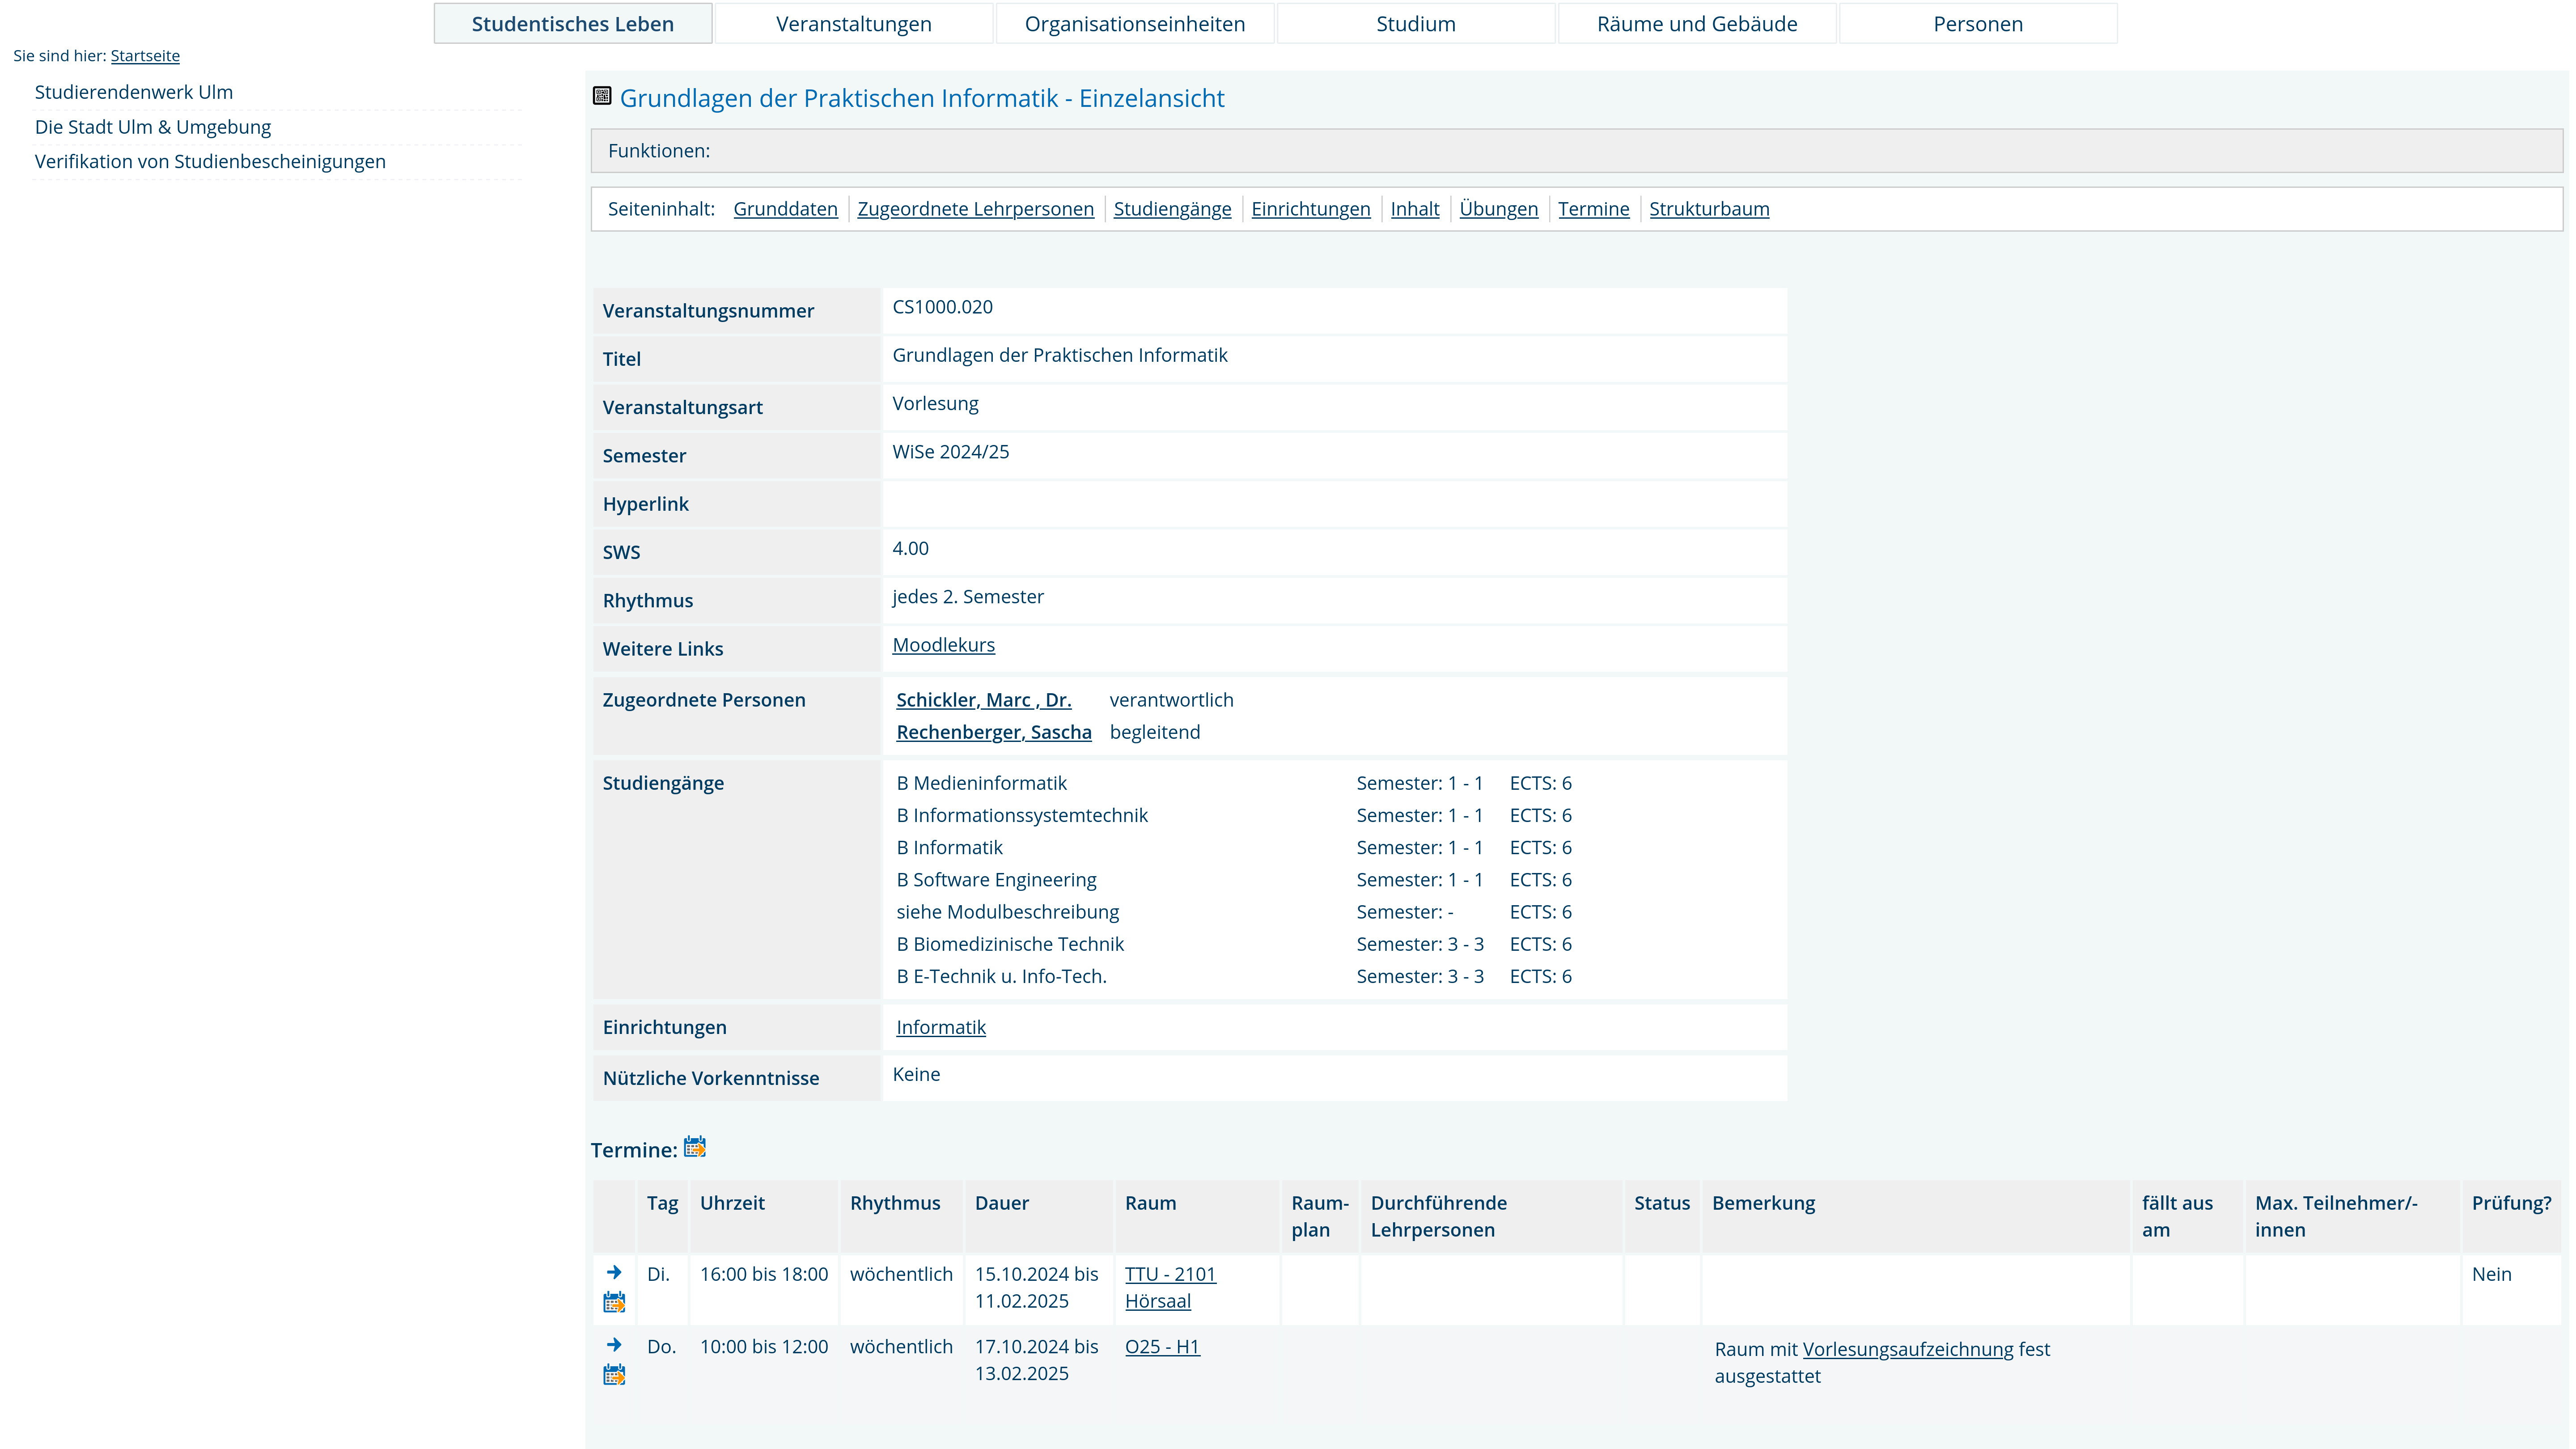
\includegraphics[clip, trim={0 10cm 0 5.5cm}, width=\linewidth]{assets/lsf-3.png}
\end{frame}

\begin{frame}{Zeitangaben}
    \begin{fancycolumns}
        \begin{definition}{sine tempore (st)}
            10 st = 10:00
        \end{definition}
        \nextcolumn
        \begin{definition}{cum tempore (ct)}
            10 ct = 10:15
        \end{definition}
    \end{fancycolumns}

    $\longrightarrow$ Die meisten Vorlesungen fangen \textbf{ct} an!
\end{frame}

\subsection{Wie finde ich den Raum meiner Vorlesung?}
\begin{frame}{\insertsubsection \space|\space Hörsaalfinder}
    \begin{fancycolumns}[widths={30}]
        \fancyqr[width=\linewidth]{https://www.uni-ulm.de/einrichtungen/kiz/weiteres/campus-navigation/hoersaalfinder/}
        
        \nextcolumn
        \centering
        \begin{minipage}[C]{0.8\textwidth}
            \begin{itemize}
                \item Hörsäle
                \item PC-Pools
                \item Drucker 
                \item Seminarräume 
            \end{itemize}
        \end{minipage}
    \end{fancycolumns}
\end{frame}

\subsection{Moodle}
\begin{frame}{\insertsubsection \space|\space\underline{\href{https://moodle.uni-ulm.de}{moodle.uni-ulm.de}}}
    \begin{itemize}
        \item Alle wichtigen Kursinformationen 
        \item Übungsblätter, Abgaben, Forum, Neuigkeiten
        \item Einschreiben in Kurse ist nicht verbindlich (Prüfungsanmeldung \underline{nur} über LSF)
    \end{itemize}
\end{frame}

\begin{frame}{\insertsubsection \space|\space\underline{\href{https://moodle.uni-ulm.de}{moodle.uni-ulm.de}}}
    \includegraphics[width=\linewidth]{assets/moodle-overview.png}
\end{frame}

\begin{frame}{\insertsubsection \space|\space\underline{\href{https://moodle.uni-ulm.de}{moodle.uni-ulm.de}}}
    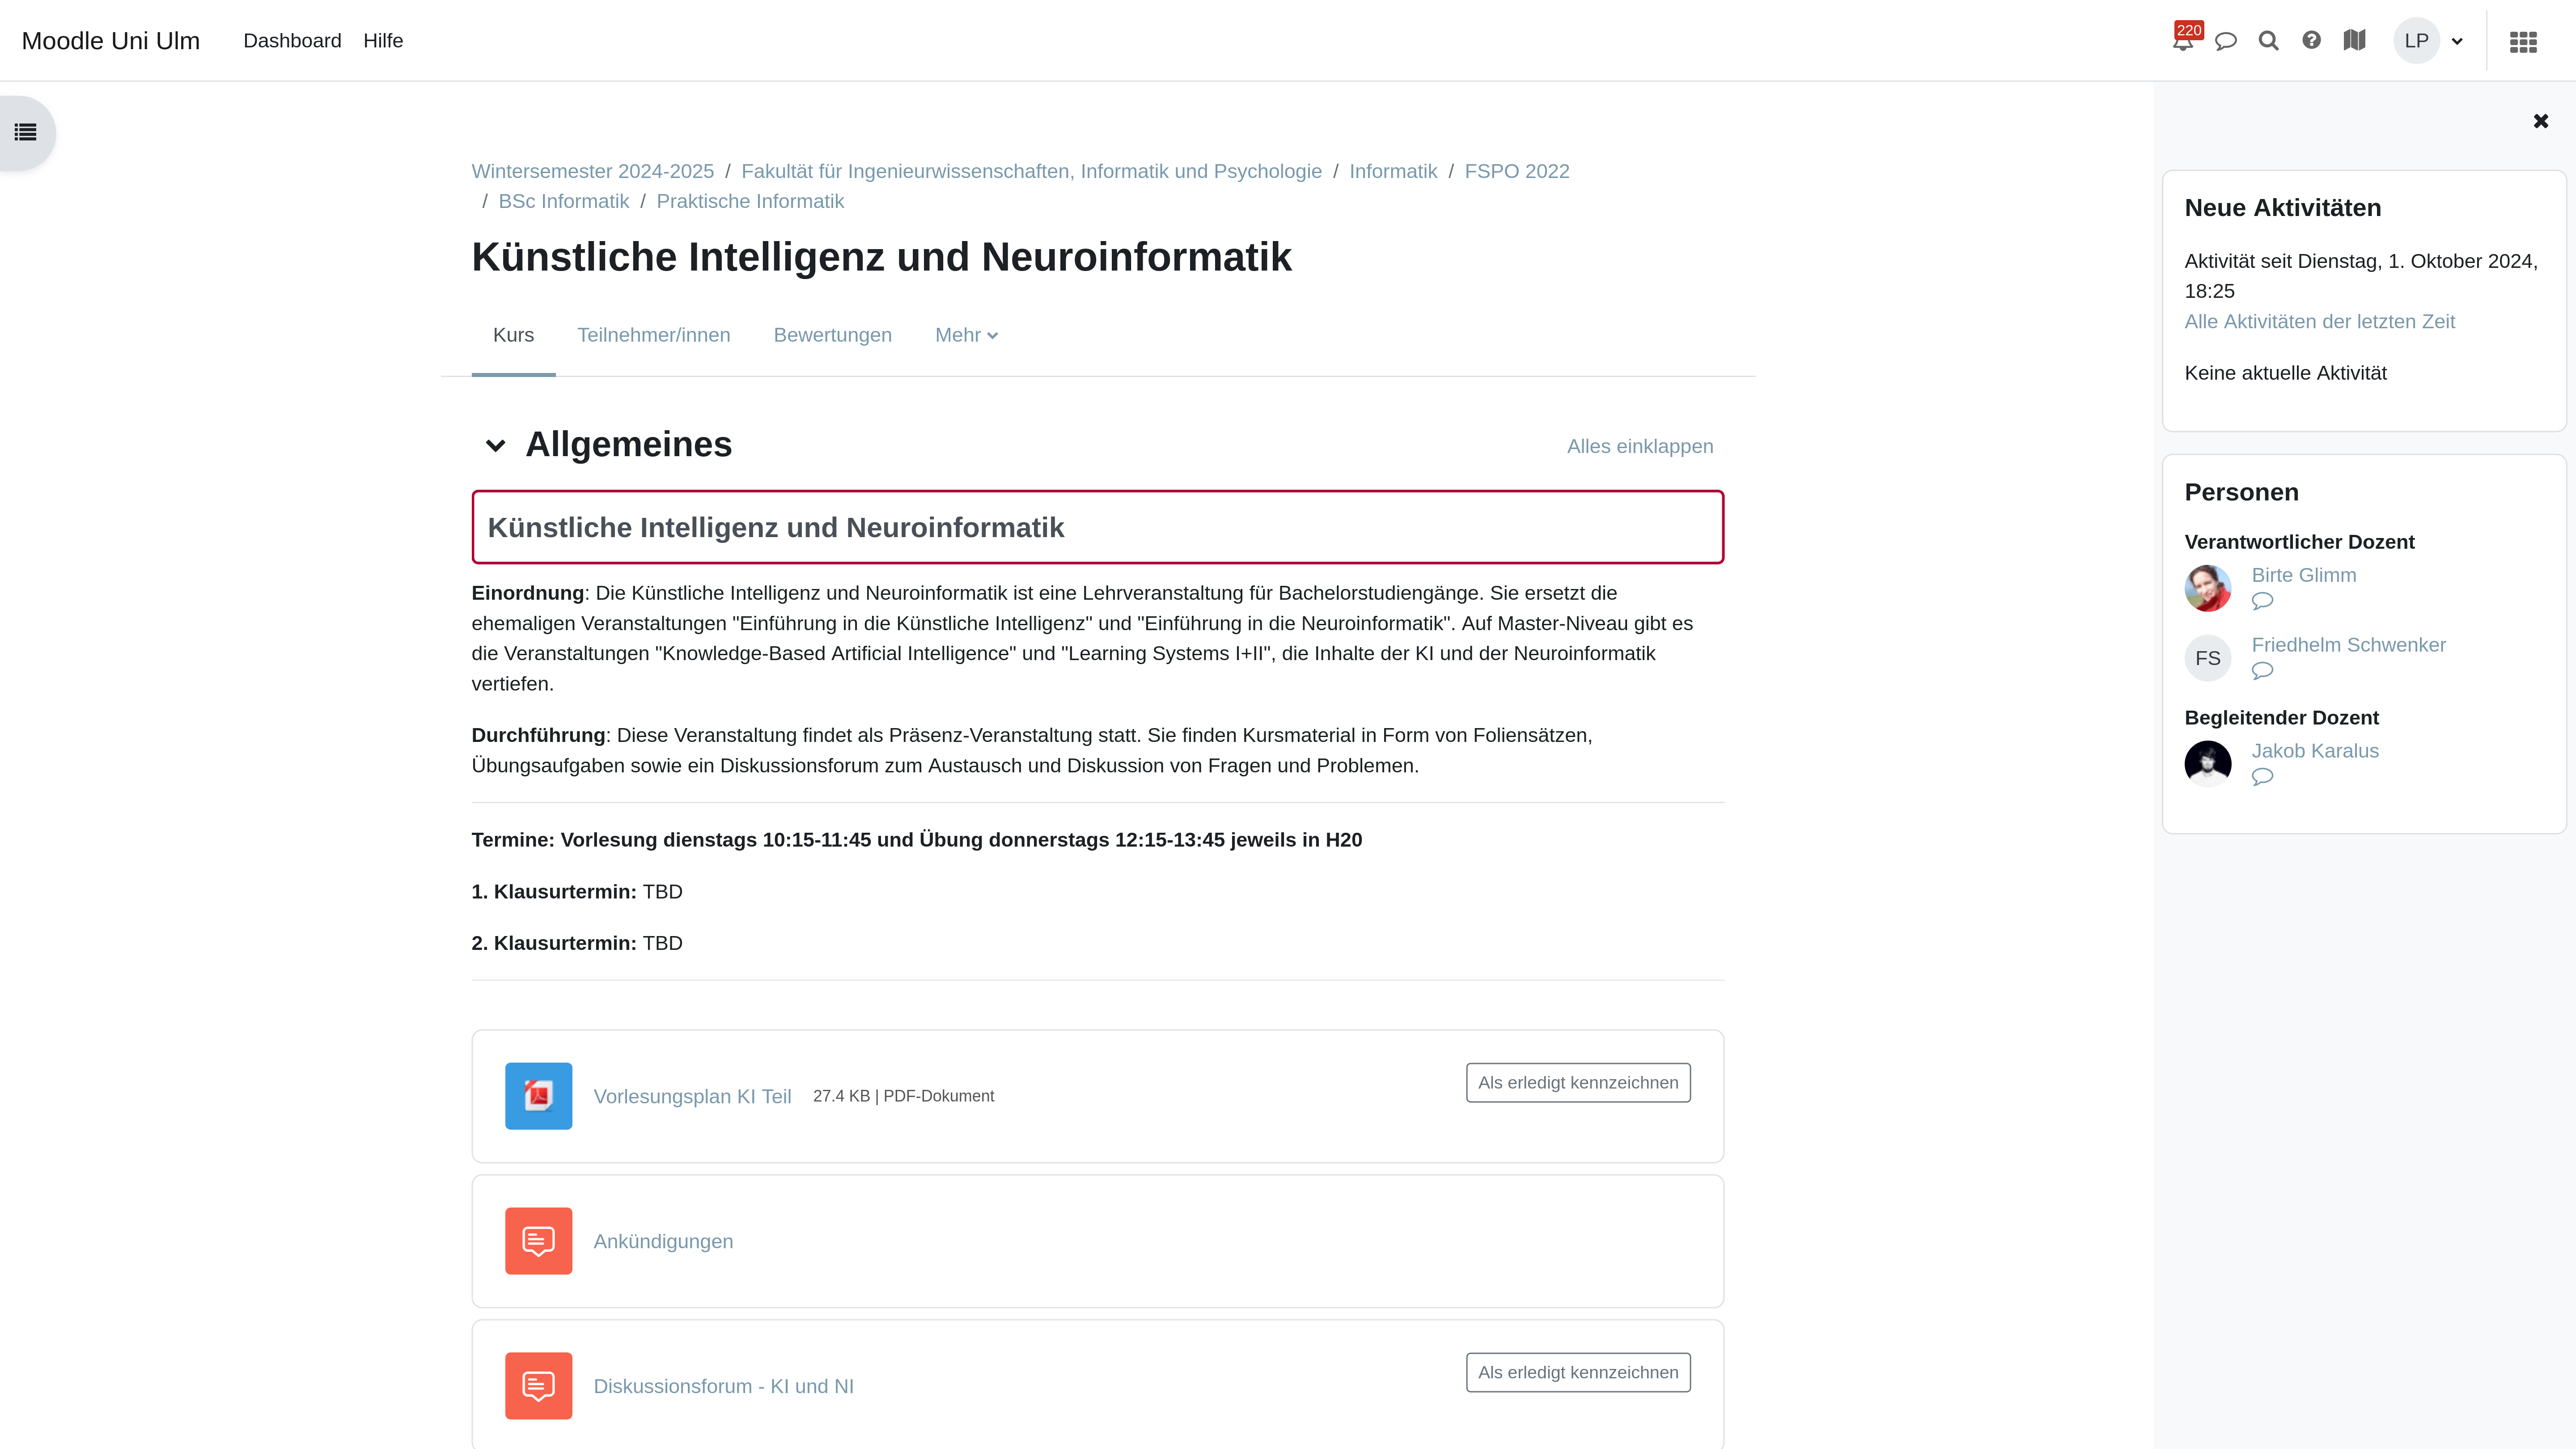
\includegraphics[width=\linewidth]{assets/moodle-course.png}
\end{frame}


\subsection{kiz Web-Services}
\begin{frame}{\insertsubsection \space|\space\underline{\href{https://portal.uni-ulm.de}{portal.uni-ulm.de}}}
    \begin{fancycolumns}[widths={60}]
        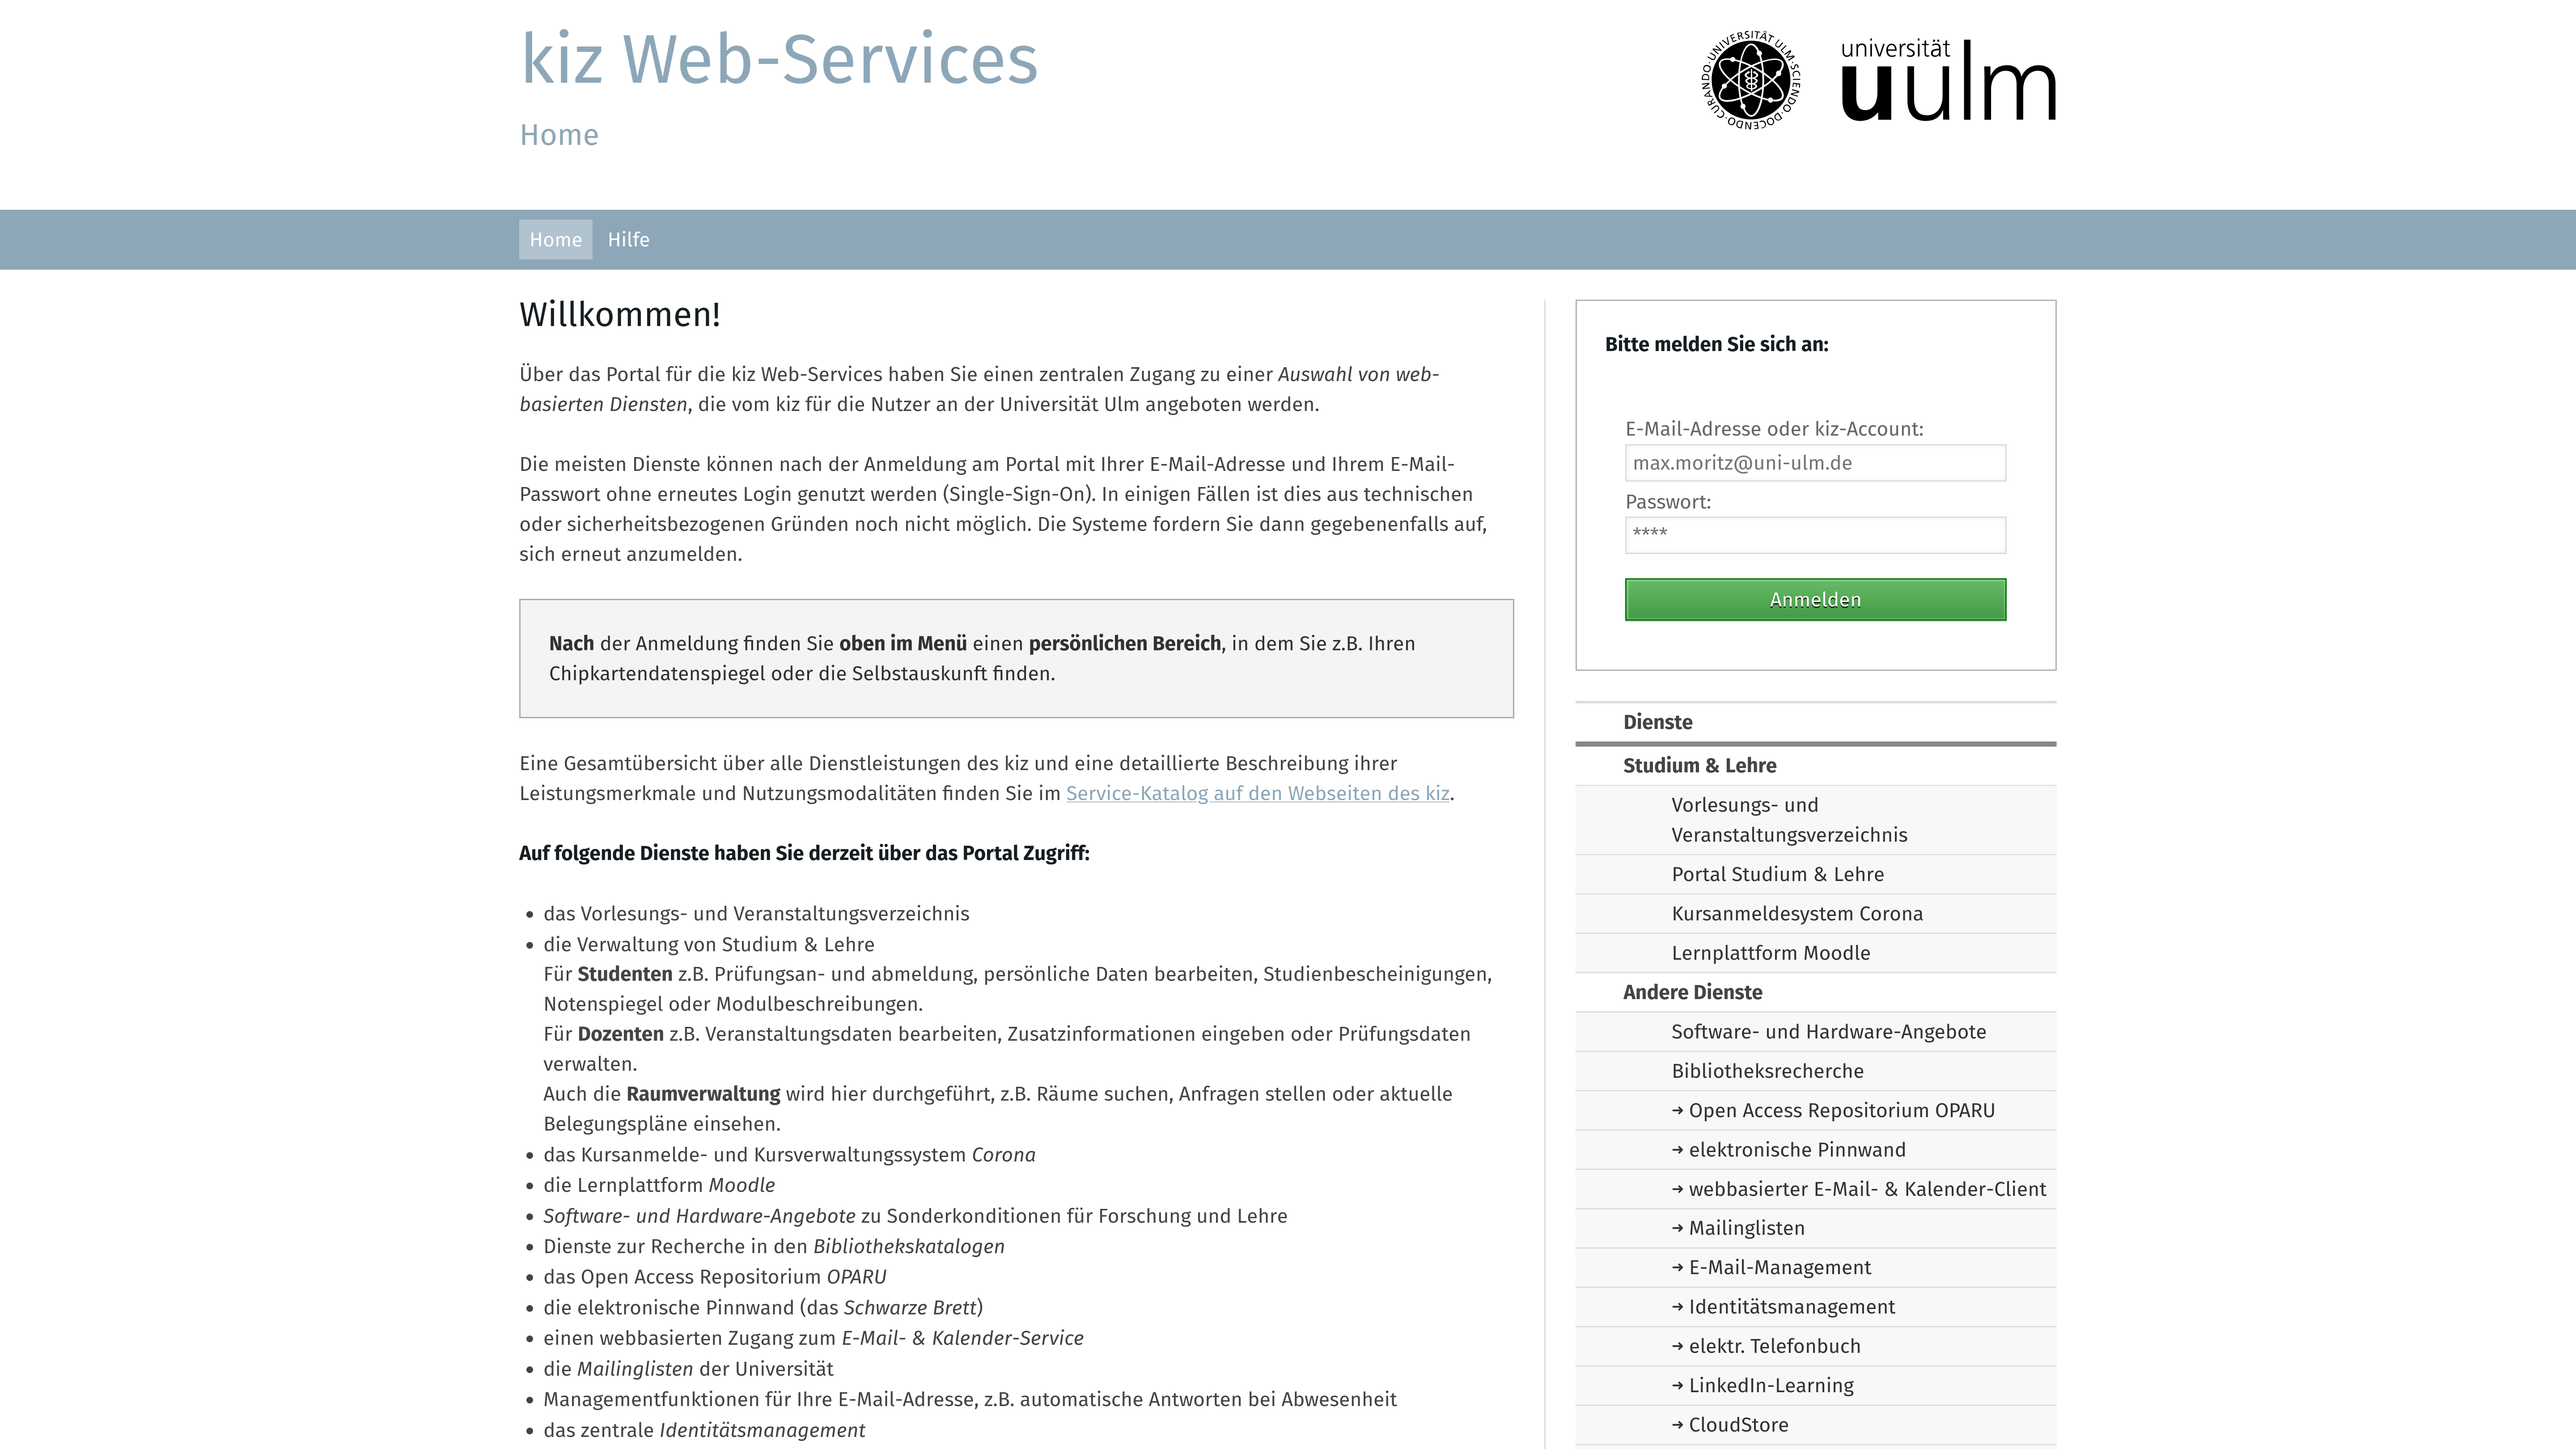
\includegraphics[clip, trim={30cm 0 30cm 0}, width=\linewidth]{assets/kiz.png}
        \nextcolumn
        \begin{itemize}
            \item Zugang zu allen Services
            \item Moodle, LSF, IDM, etc
            \item Einfache Anmeldung 
        \end{itemize}
    \end{fancycolumns}
\end{frame}

\subsection{Uni E-Mail}
\begin{frame}{\insertsubsection}
    \begin{fancycolumns}[T, widths={30}]
        \fancyqr[height=\linewidth]{https://www.uni-ulm.de/einrichtungen/kiz/service-katalog/e-mail-kalender-zusammenarbeit/e-mail/e-mail-programme-konfigurieren/}
        \begin{center}
            \textbf{Tutorial}: E-Mail-Programm konfigurieren
        \end{center}    
        \nextcolumn
        \begin{itemize}
            \item Format: \lstinline|vorname.nachname@uni-ulm.de|
            \item Wichtige Informationen und Benachrichtigungen von Moodle, LFS, etc.
            \item Über \underline{\href{https://sogo.uni-ulm.de}{sogo.uni-ulm.de}} lesen
            \item Empfehlung: \underline{\href{https://www.uni-ulm.de/einrichtungen/kiz/service-katalog/e-mail-kalender-zusammenarbeit/e-mail/e-mail-programme-konfigurieren/}{Uni Mail zur Mailapp hinzufügen}}
        \end{itemize}
    \end{fancycolumns}
\end{frame}

\section{Prüfungen}
\subsection{Wann finden Prüfungen statt?}
\begin{frame}{\insertsubsection}
    \begin{itemize}
        \item Genaues Datum im LSF, Moodle und Prüfungsplanugssystem
        \item 2 Prüfungszeiträume \footnote{\href{https://www.uni-ulm.de/fileadmin/website_uni_ulm/zuv/zuv.dezIII.abt2u3/3-2oeffentlich/bekanntmachungen/2022/veroeffentlichung_asop_final.pdf}{§20 Abs. 1 ASPO}} \begin{enumerate} 
            \item Zeitraum: Letzte Vorlesungswoche + 3 Wochen
            \item Zeitraum: 3 Wochen vor Folgesemester + 1. Vorlesungswoche
        \end{enumerate}
    \end{itemize}
    
\end{frame}


\subsection{Prüfungsplanungssystem}
\begin{frame}{\insertsubsection \space|\space \underline{\href{https://pps.informatik.uni-ulm.de/index.php}{pps.informatik.uni-ulm.de}}}
    \includegraphics[clip, trim={0 14cm 0 0}, width=\linewidth]{assets/pps.png}
\end{frame}


\subsection{Wann an/abmelden}
\begin{frame}{\insertsubsection}
    \begin{itemize}
        \item Prüfungsanmeldung im LSF (\underline{\href{https://campusonline.uni-ulm.de}{campusonline}})
        \item \textbf{Anmeldung}: Bis 5 Tage vor der schriftlichen Prüfung
        \item \textbf{Abmeldung}: Bis 1 Tag vor der schriftlichen Prüfung \footnote{\href{https://www.uni-ulm.de/fileadmin/website_uni_ulm/zuv/zuv.dezIII.abt2u3/3-2oeffentlich/bekanntmachungen/2022/veroeffentlichung_asop_final.pdf}{§ 21 Abs. 4 ASPO}}
    \end{itemize}
\end{frame}

\subsection{Prüfungs- an/abmeldung}
\begin{frame}{\insertsubsection \space|\space\underline{\href{https://campusonline.uni-ulm.de}{campusonline.uni-ulm.de}}}
    \begin{annotatedFigure}
        {\includegraphics[clip, trim={0 0 0 0}, width=\linewidth]{assets/exam.png}}
        \annotatedFigureBox{0.12,0.8287}{0.231,0.8812}{A}{0.12,0.8287}%bl
        \annotatedFigureBox{-0.004,0.7676}{0.091,0.7978}{B}{-0.004,0.7676}%bl
        \annotatedFigureBox{0.218,0.6645}{0.342,0.7071}{C}{0.218,0.6645}%bl
    \end{annotatedFigure}
\end{frame}

\subsection{CoronaNG}
\begin{frame}{\insertsubsection \space|\space\underline{\href{https://campusonline.uni-ulm.de/CoronaNG/index.html}{campusonline.uni-ulm.de/CoronaNG}}}
    \includegraphics[clip, trim={0 35cm 0 0}, width=\linewidth]{assets/coronang.png}
    $\longrightarrow$ Anmeldung für ASQ
\end{frame}

\subsection{ASPO \& FSPO}
\begin{frame}{\insertsubsection}
    \begin{fancycolumns}[T]
        \begin{definition}{\underline{\href{https://www.uni-ulm.de/fileadmin/website_uni_ulm/zuv/zuv.dezIII.abt2u3/3-2oeffentlich/bekanntmachungen/2022/veroeffentlichung_asop_final.pdf}{ASPO}}}
            \begin{itemize}
                \item Allgemeine Regeln zum Studium und Prüfungen an der Uni
                \item Gibt den Rahmen für die FSPO und die Uni vor
            \end{itemize}
        \end{definition}

        \nextcolumn
        \begin{definition}{\underline{\href{https://www.uni-ulm.de/fileadmin/website_uni_ulm/zuv/zuv.dezIII.abt2u3/3-2oeffentlich/bekanntmachungen/2022/FSPO_Informatikstudiengaenge.pdf}{FSPO}}}
            \begin{itemize}
                \item Fachspezifische Regeln zum <Studium
                \item Welche Orientierungsprüfungen man bis wann bestehen muss
                \item Wie viel Versuche für welche Prüfungen 
            \end{itemize}
        \end{definition}
    \end{fancycolumns}
    
    \begin{itemize}
        \item[$\longrightarrow$] Es lohnt sich die FSPO zu lesen / zu kennen
        \item[$\longrightarrow$] FSPO beinhaltet sehr wichtige Informationen zu Deadlines und wichtigen Prüfungen! \newline
    \end{itemize}
\end{frame}


\section{Uni, Lernen, Leben}
\subsection{Wo lernen?}
\begin{frame}{\insertsubsection}
    \begin{itemize}
        \item Lernflächen \begin{itemize} \item Überall an unserer Uni mit \textbf{LF} markiert \end{itemize}
        \item Computerpools \begin{itemize}
            \item Südpool
            \item Nordpool
            \item Smileypool \end{itemize}
        \item Bibliothek \begin{itemize} \item Möglichkeit Räume zu reservieren \end{itemize}
        \item[$\rightarrow$] Es lohnt sich Lerngruppen zu finden 
    \end{itemize}
\end{frame}

\subsection{Wie lernen?}
\begin{frame}{\insertsubsection}
    \begin{itemize}
        \item Spaced Repetition (Karteikarten) \begin{itemize}
            \item Anki, Mochi
            \item Sehr zu Empfehlen für Mathe (Definitionen Lernen)! 
            \item[$\rightarrow$] Karteikarten existieren bereist (moodle Kurs) 
        \end{itemize}
        \item Pomodoro
        \item Lerngruppen
        \item Body Doubles 
    \end{itemize}
\end{frame}

\subsection{Ansprechpersonen}
\begin{frame}{\insertsubsection}
    \begin{itemize}
        \item \underline{\textbf{\href{https://www.uni-ulm.de/studium/studienberatung/zentrale-studienberatung/}{Zentrale Studienberatung}}}: Generelle Fragen, Studiumsorganisation, Unsicherheit mit dem Studiengang, Nachteilausgleich  
        \item \underline{\textbf{\href{https://www.uni-ulm.de/studium/studienberatung/studienfachberatung/}{Studienfachberatung}}}: Spezifische Fragen zum Studiengang 
        \item \underline{\textbf{\href{https://studierendenwerk-ulm.de/}{Studierendenwerk}}}: Wohnen, Essen, Bafög, Studieren mit Kindern, Beratung
        \item \underline{\textbf{\href{https://studierendenwerk-ulm.de/beratung-betreuung/psychosoziale-beratung/}{Psychosozialberatung}}}: Kostenlos, persönliche Probleme, Lernschwierigkeiten, Prüfungsängste, etc
        \item \underline{\textbf{\href{https://stuve.uni-ulm.de/fin/aktuelles}{Fachschaft}}}: {Zusammen mit der StuVe Vertretung der Studierenden. }
        \item \textbf{Professoren}: E-Mail schreiben oder nach der Vorlesung kurz fragen
    \end{itemize}
\end{frame}

\subsection{Fachschaft Informatik (von Studierenden für Studierende)}
\begin{frame}{\insertsubsection}
    \begin{fancycolumns}[columns=2]
        \begin{definition}{Anlaufsstelle}
            \begin{itemize}
                \item Altklausuren
                \item Rat von Studierenden aus höheren Semestern
            \end{itemize}
        \end{definition}
        
        \begin{definition}{Engagement}
            \begin{itemize}
                \item Organisation von Events \begin{itemize}
                    \item Erstsemestereinführung
                    \item Uni Parties 
                    \item \dots
                \end{itemize}
                \item Mitgestaltung der Lehre
            \end{itemize}
        \end{definition}
        
        \nextcolumn
        \begin{definition}{Gemeinschaft}
            \begin{itemize}
                \item Sitzungen mit Essen
                \item Fachschaftsinterne Events 
                \item Zugang zum Fachschaftsbüro (BECI)
            \end{itemize}
        \end{definition}

        \begin{definition}{Vertretung der Studierenden}
            \begin{itemize}
                \item Vermittlung zwischen Lehrenden und Studierenden 
                \item Mitspracherecht im Prüfungsausschuss, der Studienekomission, etc.
            \end{itemize}
        \end{definition}

    \end{fancycolumns}
\end{frame}

\subsection{Wo Altklausuren?}
\begin{frame}{\insertsubsection}
    \begin{fancycolumns}[widths={30}]
        \fancyqr[width=\linewidth]{https://moodle.uni-ulm.de/course/view.php?id=53418}
        \nextcolumn

        \centering
        \begin{minipage}[C]{0.8\textwidth}
            \begin{itemize}
                \item Fachschaft Informatik
                \item[$\rightarrow$] Fachschaft Informatik Moodle Kurs 
            \end{itemize}
        \end{minipage}
    \end{fancycolumns}
\end{frame}

\subsection{Probleme mit Programmieren?}
\begin{frame}{\insertsubsection}
    \begin{fancycolumns}[widths={30}]
        \fancyqr[width=\linewidth]{https://moodle.uni-ulm.de/course/view.php?id=53212}
        \nextcolumn

        \centering
        \begin{minipage}[C]{0.8\textwidth}
            \begin{itemize}
                \item \underline{\href{https://moodle.uni-ulm.de/course/view.php?id=53212}{Programmierstarthilfe (PSH)}}
                \item Hybridveranstaltung
                \item Discord und Moodle Kurs 
                \item Haskell (Grundlagen der Praktischen Informatik)
                \item Java (Objektorientiertes Programmieren)
            \end{itemize}
        \end{minipage}
    \end{fancycolumns}
\end{frame}



\subsection{Freizeit}
\begin{frame}{\insertsubsection}
    \begin{fancycolumns}[T, columns=2]
        \begin{definition}{Sport}
            \begin{itemize}
                \item Hochschulsport (sehr viele günstige Sportkurse an der Uni)
                \item Uni Fit (Gym)
                \item Boulderhalle, Eislaufhalle, Donaubad
            \end{itemize}
        \end{definition}

        \begin{definition}{Uni}
            \begin{itemize}
                \item Uni Parties
                \item Referate (z.B. Lan-Party)
                \item Musisches Zentrum: Orchester, Chor
            \end{itemize}
        \end{definition}
        
        \nextcolumn
        \begin{definition}{Soziales}
            \begin{itemize}
                \item Studibars (quasi an jedem Wohnheim), normale Bars
                \item Roxy
                \item Events (z.B. Nabada, Lichterserenade) 
            \end{itemize}
        \end{definition}

        \begin{definition}{Kultur}
            \begin{itemize}
                \item Musen, Theater, Kinos
                \item Viele Museen kostenlos als Studi
                \item Theater vergünstigt, teilweise kostenlos
            \end{itemize}
        \end{definition}

    \end{fancycolumns}
    \dots und vieles mehr!
\end{frame}


\section{Schlussworte}
\begin{frame}{Ende}
    \begin{fancycolumns}[widths={30}]
        \fancyqr[image = \huge\faGithub, height=\linewidth]{https://github.com/FIN-Uni-Ulm/how-to-studium}
        \nextcolumn
        \begin{center}
            \LARGE{Danke für eure Aufmerksamkeit!}
        \end{center}
    \end{fancycolumns}
    
    \begin{fancycolumns}[widths={30}]
        \begin{center}
            Source \& PDF Download
        \end{center}
    \end{fancycolumns}
\end{frame}


\end{document}